\scanpage{80}

% top, lines 1–3
\[
\begin{aligned}
3)\quad n=6,\qquad &\mathbb P_6\simeq\mathbb P_3\times(\mathrm{Ens})_2\\
&\text{(marche chaque fois qu'on a $\mathbb P_n$ avec $n=2m$, $m$ impair\ldots)}\\
\text{d'où}\qquad &\mathbb P_6\simeq(\mathrm{Ens})_3\times(\mathrm{Ens})_2
\end{aligned}
\]

% upper, lines 4–7
Si $t\in(\mathrm{Ens})_{\deleted{\unsure{2}}3}$ et $\omega\in(\mathrm{Ens})_2$, \deleted{le polyg} l'hexagone associé a comme sommets les él. de $t\times\omega$, et $(a,\alpha)$ $(b,\beta)$ \deleted{\unsure{adjts}} liés sss $a\ne b$, $\alpha\ne\beta$ : \uline{L'hexagone est une bitriade}.

% upper-middle, lines 7–11
Ici, pour un hexagone donné $H$, \inserted{si $\mathrm{opp}$ est la symétrie antipodique} il y a bijection canonique entre l'ens $H_s/\mathrm{opp}\simeq\deleted{\unsure{H_t}}H_d$ des diag. et l'ens $H_{d*}$ des \deleted{\unsure{côtés}} codiag. (paires de côtés opposés) en associant à ch. diagonale la paire des $2$ côtés parallèles à celle-ci.

% middle, below paragraph
\[\boxed{H_d\simeq H_{d*}}\quad(=t)\]

% middle, lines 12–14
Soit $H_{\mathrm{tr}}$ l'ens des \inserted{$2$} ``triangles inscrits'' -- c'est $\varepsilon$\deleted{\unsure{\xi}} bien sûr, \inserted{-- ou l'ens des trièdres constituant l'hexagone --} $H_{\mathrm{tr}*}$ l'ens des triangles circonscrits

% above diagram
On a maintenant le diagramme

% left of diagram
\figure{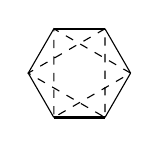
\begin{tikzpicture}[scale=.65]
\foreach \a in {0,60,120,180,240,300}{\draw (\a:1)--({\a+60}:1);}
\draw[dashed] (0:1)--(120:1)--(240:1)--cycle (60:1)--(180:1)--(300:1)--cycle;
\draw[thick] (60:1)--(120:1) (240:1)--(300:1);
\end{tikzpicture}}

% middle-lower, diagram
\diagram{\begin{tikzcd}[ampersand replacement=\&,row sep=1em,column sep=1.5em,cells={font=\scriptsize}]
\& H_s\arrow[ddl,"2" description,"\mathrm{opp}"']\arrow[ddd,"3"]\&\&H_r\,D_6\arrow[ll,"2"']\arrow[dll,"2" description,"\mathrm{opp}"']\arrow[ddl,"2"]\arrow[ddd,"3"]\\
\&H_{r'}\,\mathfrak S_3\arrow[dl,"2"]\arrow[ddd]\&\&\\
H_d\arrow[ddd,"3"']\&\&H_{s*}\arrow[ll,"2" description,"\mathrm{opp}"]\arrow[ddd,"3"]\&\\
\&H_{\mathrm{tr}}\arrow[ddl,"2"']\&\&H_{\mathrm{tror}}\,\mathbb F_2^2\arrow[ll,"2"']\arrow[dll,"2"]\arrow[ddl,"2"]\\
\&H_\omega\arrow[dl,"2"']\&\&\\
e\&\&H_{\mathrm{tr}*}\arrow[ll,"2"']\&
\end{tikzcd}}

% right of diagram
\margin{\uline{NB} tous les carrés cart. toutes les fl. hor. de degré $2$ \rule{2em}{.3pt} vert \rule{2em}{.3pt} $3$}

% below diagram, four braced notes
\[
\mathrm{Nb}\ \left\{\begin{aligned}
H_d&=\text{ens des sommets d'un triangle inscrit ou circonscrit}\\
H_\omega&=\text{ens des orientations de }H\simeq\omega(H_d)\simeq H_{\mathrm{tr}}\wedge H_{\mathrm{tr}*}\\
H_{r'}&=H_r/\mathrm{opp}\simeq\text{ens des rep. de }H_d\text{ (donc $\mathfrak S_3$-torseur)}\\
H_{\mathrm{tr}}\times H_{\mathrm{tr}*}&\simeq H_{\mathrm{tr}}\times H_\omega\simeq H_{\mathrm{tror}}\quad\text{ens des 4 triangles \unsure{inscrit|inscrits} \uline{orientés}}
\end{aligned}\right.
\]

% foot, lines 1–6
Ceci correspond au diagramme des sous groupes de
\[
D_6=\mathfrak S_2\mathbin{.}\mathbb Z/6\mathbb Z\simeq\mathfrak S_2\times\mathfrak S_3\quad\text{d'ordre }12.\quad D_6.
\]
ayant \inserted{trois} \deleted{\unsure{un}} sous-groupes \inserted{(conjugués)} d'indice $3$ (stabilisateurs des \inserted{trois} él. de $H_d$) $3$ sous-groupes \inserted{(deux à deux \inserted{non} conjugués)} d'indices $2$ (stabilisateurs des él. de $H_{\mathrm{tr}},H_{\mathrm{tr}*},H_\omega$ respectivement), un sous-gpe d'indice $4$ (stabilisateur des él. de $H_{\mathrm{tror}}$)

% archive sheet number: 79
